\newgeometry{top=1cm, bottom=2cm}
\section{Lineare Abbildungen}
\begin{figure}[h!]
    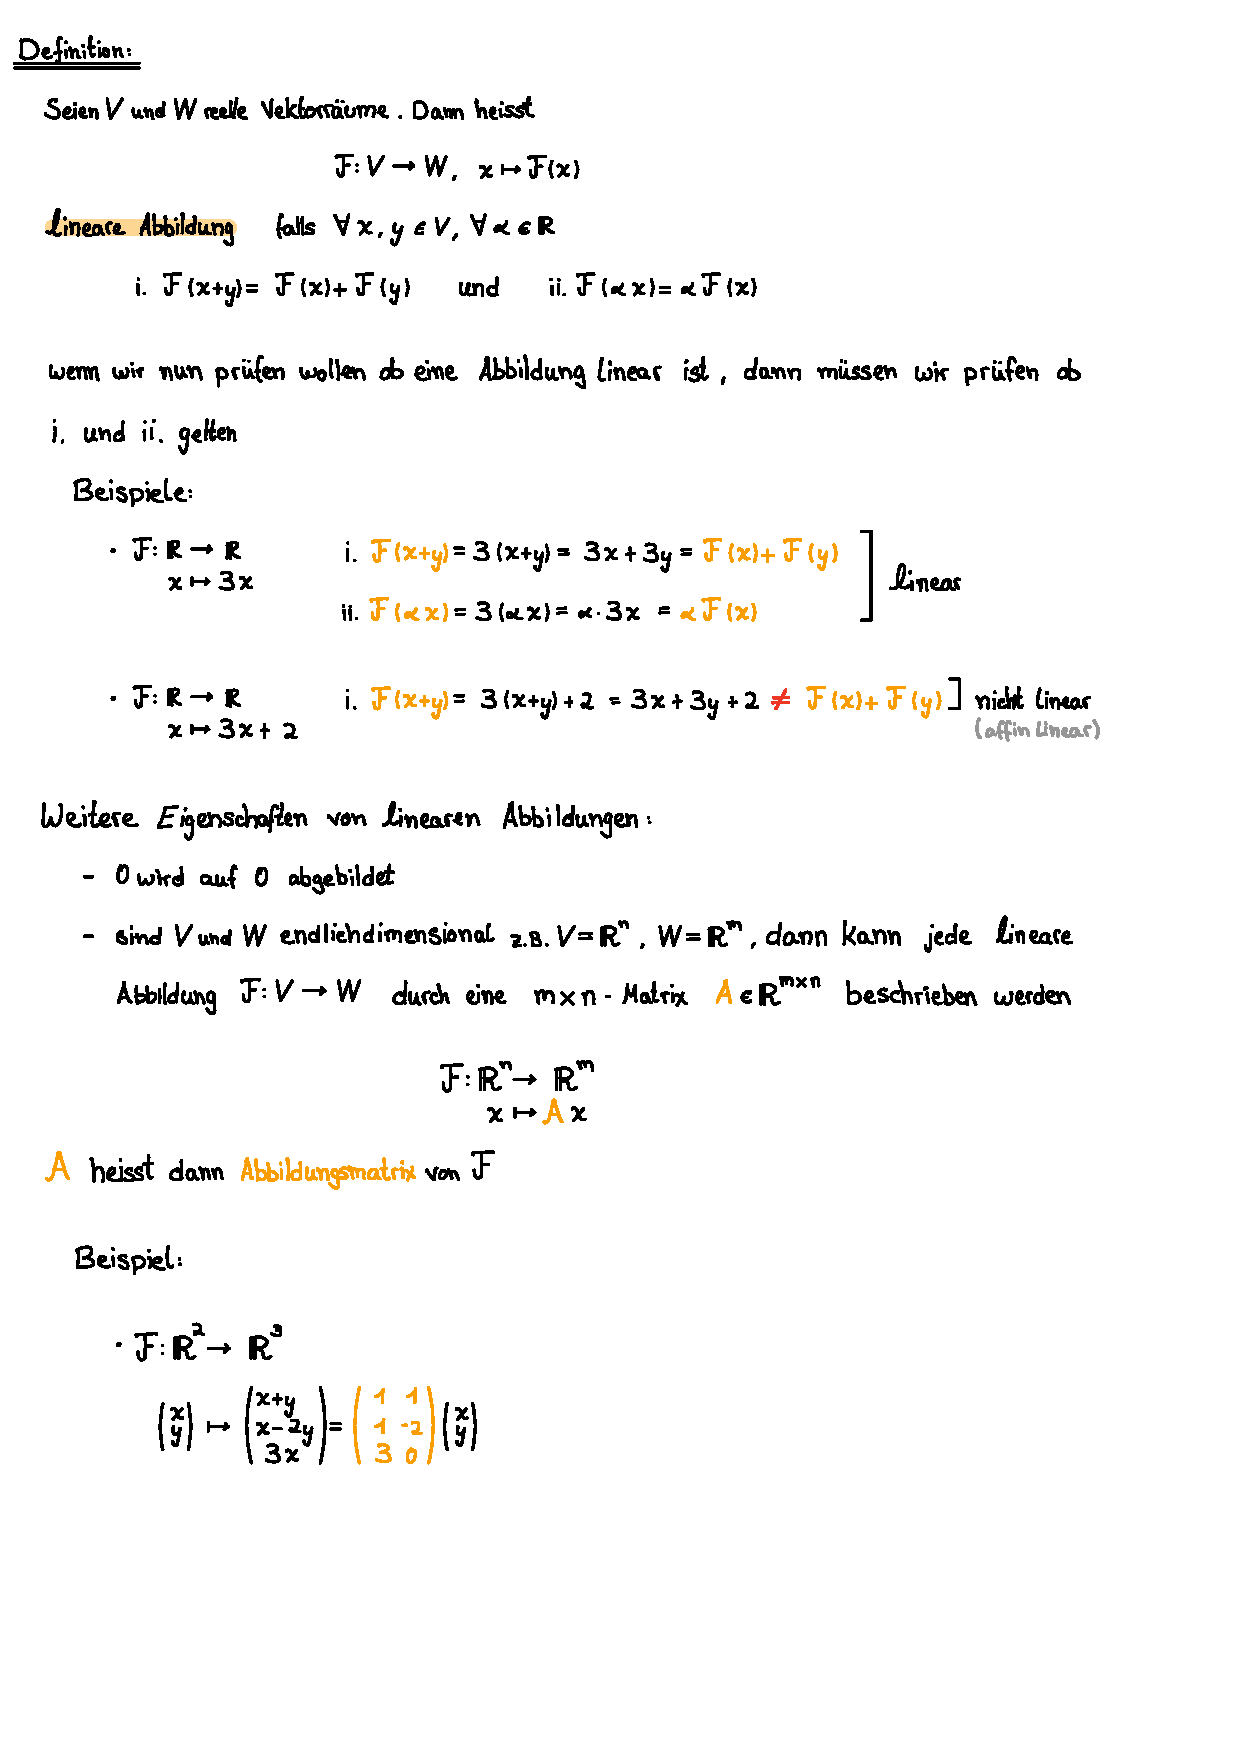
\includegraphics[page=1, scale=0.842]{pdf/05_Lineare_Abbildungen.pdf}
\end{figure}
\newpage
\includepdf[pages={2-}, 
            pagecommand={\thispagestyle{plain}}, 
            scale=0.95]{pdf/05_Lineare_Abbildungen.pdf}

\newgeometry{top=2.5cm, bottom=2cm}

\subsection{Beispielaufgaben} %Übung 01

\vspace{1cm}

\subsubsection{} %serie 06
Sei
\begin{equation*}
    A = \begin{pmatrix}
    2 & 1 & -1 & 2 \\
    1 & 0 & -1 & 0 \\
    3 & 1 & -2 & 2 \\
    \end{pmatrix}.
\end{equation*}

Bestimmen Sie eine Basis für das Bild und den Kern von \( A \).

\vspace{1\baselineskip}

\begin{solution}   

    \leftskip=2em

    \begin{equation*}
        \begin{gmatrix}[L]
            2 & 1 & -1 & 2 \\
            1 & 0 & -1 & 0 \\
            3 & 1 & -2 & 2 
        \end{gmatrix} \hspace{-0.75em} \begin{gmatrix}[R]
            0 \\ 0 \\ 0
                \rowops
                    \swap{0}{1}
        \end{gmatrix} \rightarrow \; \begin{gmatrix}[L]
            1 & 0 & -1 & 0 \\
            2 & 1 & -1 & 2 \\
            3 & 1 & -2 & 2 
        \end{gmatrix} \hspace{-0.75em} \begin{gmatrix}[R]
            0 \\0 \\ 0
                \rowops
                    \add[-2]{0}{1}
                    \add[-3]{0}{2}
        \end{gmatrix} \rightarrow \; \begin{gmatrix}[L]
            1 & 0 & -1 & 0 \\
            0 & 1 & 1 & 2 \\
            0 & 1 & 1 & 2
        \end{gmatrix} \hspace{-0.75em} \begin{gmatrix}[R]
            0 \\0 \\ 0
                \rowops
                    \add[-1]{1}{2}
        \end{gmatrix}
    \end{equation*}

    \begin{equation*}
        \begin{gmatrix}[L]
            1 & 0 & -1 & 0 \\
            0 & 1 & 1 & 2 \\
            0 & 0 & 0 & 0
        \end{gmatrix} \hspace{-0.75em} \begin{gmatrix}[R]
            0 \\0 \\ 0
        \end{gmatrix} \: \begin{aligned}
            x_4 &= t \\
            x_3 &= s \\
            x_2 &= -s - 2t \\
            x_1 &= s
        \end{aligned} \; \rightarrow \begin{pmatrix}
            s \\ -s - 2t \\ s \\ t
        \end{pmatrix}, \; \text{Kern}(A) = \left\{ \begin{pmatrix}
            1 \\ -1 \\ 1 \\ 0
        \end{pmatrix}, \begin{pmatrix}
            0 \\ -2 \\ 0 \\ 1
        \end{pmatrix} \right\}.
    \end{equation*}

    Da Rang\( (A) = 2 \), nehmen wir zwei linear unabhängige Spaltenvektoren von \( A \) als Basis für das Bild:

    \begin{equation*}
        \text{Bild}(A) = \left\{ \begin{pmatrix}
            2 \\ 1 \\ 3
        \end{pmatrix}, \begin{pmatrix}
            1 \\ 0 \\ 1
        \end{pmatrix} \right\}.
    \end{equation*}

\end{solution}

\subsubsection{} %Prüfiung S.12

Sei \( \mathcal{P}_2 \) der Vektorraum der Polynome vom Grad \( \leq 2 \) mit der Basis \( \mathcal{B} = \{1,x,x^2\} \). Sei
\begin{equation*}
    \begin{aligned}
        \mathcal{L}: \; \mathcal{P}_2 &\rightarrow \mathcal{P}_2 \\
        p(x) &\mapsto p''(x)+4p'(x)+3p(x)
    \end{aligned}
\end{equation*}

Bestimmen Sie die Darstellungsmatrix von \( \mathcal{L} \) bezüglich der Basis \( \mathcal{B} \).

\vspace{1\baselineskip}

\begin{solution}    

    \vspace{1\baselineskip}

    \leftskip=2em

    \begin{equation*}
        \begin{aligned}
            1 &= \begin{pmatrix} 1 \\ 0 \\ 0\end{pmatrix} \xrightarrow{\mathcal{L}} 3 &= \begin{pmatrix}3 \\ 0 \\ 0 \end{pmatrix} \ \text{1. Spalte von} \ A \\
            x &= \begin{pmatrix} 0 \\ 1 \\ 0\end{pmatrix} \xrightarrow{\mathcal{L}} 4+3x &= \begin{pmatrix} 4 \\ 3 \\ 0 \end{pmatrix} \ \text{2. Spalte von} \ A \\
            x^2 &= \begin{pmatrix} 0 \\ 0 \\ 1\end{pmatrix} \xrightarrow{\mathcal{L}} 2+8x+3x^2 &= \begin{pmatrix} 2 \\ 8 \\ 3 \end{pmatrix} \ \text{3. Spalte von} \ A
        \end{aligned}
    \end{equation*}

\end{solution}

\newpage

\subsubsection{}

Geben seinen die Abbildungen

\begin{enumerate}[label=\alph*)]
    \item \( \mathcal{F}: \mathbb{R}^2 \rightarrow \mathbb{R}^2,\; (x_1,x_2)^\top \mapsto (2x_1+x_2,x_1)^\top \)
    \item \( \mathcal{G}: \mathcal{C} ([x_0,x_1], \mathbb{R}) \rightarrow \mathbb{R},\; g(x) \mapsto \int_{x_0}^{x_1} g(x) \,dx \)
\end{enumerate}

Prüfe, ob die Abbildungen \( \mathcal{F,G} \) linear sind.

\vspace{1\baselineskip}

\textit{Tipp}: \( \mathcal{C} ([x_0,x_1], \mathbb{R}) \) beschreibt alle stetigen Funktionen auf dem Intervall \( [x_0,x_1] \). 

\vspace{1\baselineskip}

\begin{solution}    

    \vspace{1\baselineskip}

    \leftskip=2em

    \textbf{a)} 

    \begin{equation*}
        \begin{aligned}
            \mathcal{F}(x+y) &= \begin{pmatrix}
                2(x_1+y_1)+x_2+y_2 \\
                x_1+y_1
            \end{pmatrix} = \begin{pmatrix}
                2x_1+x_2 \\
                x_1
            \end{pmatrix} + \begin{pmatrix}
                2y_1+y_2 \\
                y_1
            \end{pmatrix} \\
            &= \mathcal{F}(x) + \mathcal{F}(y) \\[0.5em]
            \mathcal{F}(\alpha x) &= \begin{pmatrix}
                \alpha 2 x_1+\alpha x_2 \\
                \alpha x_1
            \end{pmatrix} = \alpha \begin{pmatrix}
                2x_1+x_2 \\
                x_1
            \end{pmatrix} = \alpha \mathcal{F}(x)
        \end{aligned}
    \end{equation*}

    \( \mathcal{F} \) ist linear.

    \vspace{1\baselineskip}

    \textbf{b)}

    \begin{equation*}
        \begin{aligned}
            \mathcal{G}(g+h) &= \int_{x_0}^{x_1} g(x)+h(x) \,dx = \int_{x_0}^{x_1} g(x) \,dx + \int_{x_0}^{x_1} h(x) \,dx \\
            &= \mathcal{G}(g) + \mathcal{G}(h) \\[0.5em]
            \mathcal{G}(\alpha g) &= \int_{x_0}^{x_1} \alpha g(x) \,dx = \alpha \int_{x_0}^{x_1} g(x) \,dx = \alpha \mathcal{G}(g)
        \end{aligned}
    \end{equation*}

    \( \mathcal{G} \) ist linear.

\end{solution}

% \newpage
% \subsubsection{}
% Sei $V = \mathcal{P}_2$ und $W = \mathcal{P}_1$. Wobei V durch die Basis $\mathcal{B} = (1,x,x^2)$ und $W$ durch die Basis $\mathcal{C} = (1,x)$ beschrieben werden kann. sei ausserdem
% \[\begin{aligned}
% \mathcal{F}: \; V &\rightarrow W \\
% p(x) &\mapsto p'(x)+p''(x)
% \end{aligned}\]
% Bestimme die Abbildungsmatrix $A$ der Abbildung $\mathcal{F}$. \\

% \noindent \textbf{Lösung:}

\newpage

\subsubsection{} %Serie 06

Gegeben Sei der Vektorraum \( V = \mathbb{R}^3 \) mit der Standardbasis \( \mathcal{B} \). Die Matrix

\begin{equation*}
    A = \begin{pmatrix}
    -\frac{5}{6} & \frac{1}{6} & \frac{1}{3} \\
    \frac{1}{6}  & -\frac{5}{6} & \frac{1}{3} \\
    \frac{1}{3} & \frac{1}{3} & -\frac{1}{3} \\
    \end{pmatrix}.
\end{equation*}

definiert eine lineare Abbildung von \( V \) nach \( V \).

\begin{enumerate}[label=\alph*)]
    \item Durch eine Wahl der neuen Basis
           \begin{equation*} 
                \mathcal{B}' = \left\{ 
                \begin{pmatrix}
                    2\\ 0\\ -1\\
                \end{pmatrix}, \begin{pmatrix}
                    -1\\ 1\\ 0\\
                \end{pmatrix}, \begin{pmatrix}
                    1\\ 1\\ 2\\
                \end{pmatrix}
                    \right\}.
            \end{equation*}
        werden neue Koordinaten eingeführt. Bestimmen Sie die Übergangsmatrix \( T \) von \( \mathcal{B}\) nach \( \mathcal{B}' \).
    \item Durch welche Matrix \( B \) wird die lineare Abbildung in den neuen Koordinaten \( \mathcal{B}'\) beschrieben?
\end{enumerate}

\vspace{1\baselineskip}

\begin{solution}    

    \vspace{1\baselineskip}

    \leftskip=2em

    \textbf{a)} \( \quad T_{\mathcal{B'} \to \mathcal{B}} \equiv S = \begin{pmatrix}
            2 & -1 & 1 \\
            0 & 1 & 1 \\
            -1 & 0 & 2
        \end{pmatrix}, \ T = S^{-1} = \begin{pmatrix}
            2 & -1 & 1 \\
            0 & 1 & 1 \\
            -1 & 0 & 2
        \end{pmatrix}^{-1} \)

    \vspace{0.5\baselineskip}

    \( S^{-1} \) mit Gauss-Jordan bestimmen:

    \begin{equation*}
        \begin{gmatrix}[E]
            2 & -1 & 1 \\
            0 & 1 & 1 \\
            -1 & 0 & 2
        \end{gmatrix} \hspace{-0.75em} \begin{gmatrix}[D]
            1 & 0 & 0 \\
            0 & 1 & 0 \\
            0 & 0 & 1
        \end{gmatrix} \rightarrow \begin{gmatrix}[E]
            1 & -\frac{1}{2} & \frac{1}{2} \\
            0 & 1 & 1 \\
            0 & -\frac{1}{2} & \frac{5}{2}
        \end{gmatrix} \hspace{-0.75em} \begin{gmatrix}[D]
            \frac{1}{2} & 0 & 0 \\
            0 & 1 & 0 \\
            \frac{1}{2} & 0 & 1
        \end{gmatrix} \rightarrow \begin{gmatrix}[E]
            1 & -\frac{1}{2} & \frac{1}{2} \\
            0 & 1 & 1 \\
            0 & 0 & 3
        \end{gmatrix} \hspace{-0.75em} \begin{gmatrix}[D]
            \frac{1}{2} & 0 & 0 \\
            0 & 1 & 0 \\
            \frac{1}{2} & \frac{1}{2} & 1
        \end{gmatrix} 
    \end{equation*}

    \begin{equation*}
        \begin{gmatrix}[E]
            1 & 0 & 1 \\
            0 & 1 & 1 \\
            0 & 0 & 1
        \end{gmatrix} \hspace{-0.75em} \begin{gmatrix}[D]
            \frac{1}{2} & \frac{1}{2} & 0 \\
            0 & 1 & 0 \\
            \frac{1}{6} & \frac{1}{6} & \frac{1}{3}
        \end{gmatrix} \rightarrow \begin{gmatrix}[E]
            1 & 0 & 0 \\
            0 & 1 & 0 \\
            0 & 0 & 1
        \end{gmatrix} \hspace{-0.75em} \begin{gmatrix}[D]
            \frac{1}{3} & \frac{1}{3} & -\frac{1}{3} \\
            -\frac{1}{6} & \frac{5}{6} & -\frac{1}{3} \\
            \frac{1}{6} & \frac{1}{6} & \frac{1}{3}
        \end{gmatrix} \rightarrow T = \begin{pmatrix}
            \frac{1}{3} & \frac{1}{3} & -\frac{1}{3} \\
            -\frac{1}{6} & \frac{5}{6} & -\frac{1}{3} \\
            \frac{1}{6} & \frac{1}{6} & \frac{1}{3}
        \end{pmatrix}
    \end{equation*}

    \vspace{1\baselineskip}

    \textbf{b)} \( \qquad B = T [A]_{\mathcal{B}} S \)

    \begin{equation*}
        B = \begin{pmatrix}
            \frac{1}{3} & \frac{1}{3} & -\frac{1}{3} \\
            -\frac{1}{6} & \frac{5}{6} & -\frac{1}{3} \\
            \frac{1}{6} & \frac{1}{6} & \frac{1}{3}
        \end{pmatrix} \begin{pmatrix}
            -\frac{5}{6} & \frac{1}{6} & \frac{1}{3} \\
            \frac{1}{6}  & -\frac{5}{6} & \frac{1}{3} \\
            \frac{1}{3} & \frac{1}{3} & -\frac{1}{3} \\
        \end{pmatrix} \begin{pmatrix}
            2 & -1 & 1 \\
            0 & 1 & 1 \\
            -1 & 0 & 2
        \end{pmatrix} = \begin{pmatrix}
            -1 & 0 & 0 \\
            0 & -1 & 0 \\
            0 & 0 & 0 \\
        \end{pmatrix}
    \end{equation*}

\end{solution}

\newpage

\subsubsection{} %Zardini S.84

Betrachten Sie die Abbildung \( \mathcal{F}: \mathbb{R}^3 \rightarrow \mathbb{R}^3 \) gegeben durch

\begin{equation*}
    \begin{pmatrix}
    x\\
    y\\
    z\\
    \end{pmatrix} \mapsto
    \begin{pmatrix}
    7x+5y-8z\\
    5x+3y-4z\\
    -x-3y+8z\\
    \end{pmatrix}
\end{equation*}

\begin{enumerate}[label=\alph*)]
    \item Geben Sie die Darstellungsmatrix von \( \mathcal{F} \) bezüglich der Standardbasis \( \mathcal{E} = \{e_1,e_2,e_3\} \) von \( \mathbb{R}^3 \) an.
    \item Berechnen Sie die Darstellungsmatrix von $\mathcal{F}$ bezüglich $\mathcal{B}$ unter Verwendung der Übergangsmatrix $T$ und ihrer Inversen.
    \item Gegeben sei die Basis \( \mathcal{B} = \{b_1 := e_1,\; b_2 :=e_1+e_2,\; b_3 := e_2+e_3 \} \) von \( \mathbb{R}^3 \). Finden Sie die Übergangsmatrix \( T \) von \( \mathcal{B} \) nach \( \mathcal{E} \) und ihre Inverse \( T^{-1} \).
    \item Bestimmen Sie eine Basis des Kerns von \( \mathcal{F} \) und eine Basis des Bildes von \( \mathcal{F} \). Geben Sie ausserdem die jeweiligen Dimensionen an.
\end{enumerate}

\vspace{1\baselineskip}

\begin{solution}    

    \vspace{1\baselineskip}

    \leftskip=2em

    \textbf{a)} \( \ [\mathcal{F}]_{\mathcal{E}} = \begin{pmatrix}
        7 & 5 & -8 \\
        5 & 3 & -4 \\
        -1 & -3 & 8
    \end{pmatrix} \)

    \vspace{1\baselineskip}

    \textbf{b)} \( \ T_{\mathcal{B} \to \mathcal{E}} = \begin{pmatrix}
        1 & 1 & 0 \\
        0 & 1 & 1 \\
        0 & 0 & 1
    \end{pmatrix} \)

    \begin{equation*}
        \begin{gmatrix}[E]
            1 & 1 & 0 \\
            0 & 1 & 1 \\
            0 & 0 & 1
        \end{gmatrix} \hspace{-0.75em} \begin{gmatrix}[D]
            1 & 0 & 0 \\
            0 & 1 & 0 \\
            0 & 0 & 1
        \end{gmatrix} \rightarrow \begin{gmatrix}[E]
            1 & 1 & 0 \\
            0 & 1 & 0 \\
            0 & 0 & 1
        \end{gmatrix} \hspace{-0.75em} \begin{gmatrix}[D]
            1 & 0 & 0 \\
            0 & 1 & -1 \\
            0 & 0 & 1
        \end{gmatrix} \rightarrow \begin{gmatrix}[E]
            1 & 0 & 0 \\
            0 & 1 & 0 \\
            0 & 0 & 1
        \end{gmatrix} \hspace{-0.75em}\underbrace{\begin{gmatrix}[D]
            1 & -1 & 1 \\
            0 & 1 & -1 \\
            0 & 0 & 1
        \end{gmatrix}}_{T_{\mathcal{E} \to \mathcal{B}}} \hspace{-1.75cm}
    \end{equation*}

    \textbf{c)} \( \ [\mathcal{F}]_{\mathcal{B}} = T_{\mathcal{E} \to \mathcal{B}} [\mathcal{F}]_{\mathcal{E}} T_{\mathcal{B} \to \mathcal{E}} \)

    \begin{equation*}
        = \begin{pmatrix}
            1 & -1 & 1 \\
            0 & 1 & -1 \\
            0 & 0 & 1
        \end{pmatrix} \begin{pmatrix}
            7 & 5 & -8 \\
            5 & 3 & -4 \\
            -1 & -3 & 8
        \end{pmatrix} \begin{pmatrix}
            1 & 1 & 0 \\
            0 & 1 & 1 \\
            0 & 0 & 1
        \end{pmatrix} = \begin{pmatrix}
            1 & 0 & 3 \\
            6 & 12 & -6 \\
            -1 & -4 & 5
        \end{pmatrix} \hspace{-2.18cm}
    \end{equation*}

    \textbf{d)} 

    \begin{equation*}
        \begin{gmatrix}[L]
            7 & 5 & -8 \\
            5 & 3 & -4 \\
            -1 & -3 & 8
        \end{gmatrix} \hspace{-0.75em} \begin{gmatrix}[R]
            0 \\ 0 \\ 0
        \end{gmatrix} \rightarrow \begin{gmatrix}[L]
            1 & 3 & -8 \\
            0 & -12 & 36 \\
            0 & -16 & 48
        \end{gmatrix} \hspace{-0.75em} \begin{gmatrix}[R]
            0 \\ 0 \\ 0
        \end{gmatrix} \rightarrow \begin{gmatrix}[L]
            1 & 0 & 1 \\
            0 & 1 & -3 \\
            0 & 0 & 0
        \end{gmatrix} \hspace{-0.75em} \begin{gmatrix}[R]
            0 \\ 0 \\ 0
        \end{gmatrix} \rightarrow \ \begin{aligned}
            x_3 &= t \\
            x_2 &= 3t \\
            x_1 &= -t
        \end{aligned}
    \end{equation*}

    Da \( \text{Rang}(\mathcal{F}) = 2 \) ist, hat das Bild die Dimension 2. Für eine Basis des Bildes nehmen wir zwei linear unabhängige Spaltenvektoren von \( \mathcal{F} \):

    \begin{equation*}
        \text{Bild}(\mathcal{F}) = \left\{ \begin{pmatrix}
            7 \\ 5 \\ -1
        \end{pmatrix}, \begin{pmatrix}
            5 \\ 3 \\ -3
        \end{pmatrix} \right\}, \quad \text{Kern}(\mathcal{F}) = \left\{ \begin{pmatrix}
            -1 \\ 3 \\ 1
        \end{pmatrix} \right\}.
    \end{equation*}

    Die Dimensionen sind dann \( \text{dim(Bild}(\mathcal{F})) = 2 \) und \( \text{dim(Kern}(\mathcal{F})) = 1 \).

\end{solution}